\documentclass[a4paper,12pt]{article}

\usepackage[utf8]{inputenc}
\usepackage[T1]{fontenc}
\usepackage{cmap}
\usepackage[english]{babel}

\newcommand{\protocol}{Solver performance measurement}
\newcommand{\labtitle}{DUVOD @ FI MU}
\newcommand{\authorname}{Boris Parák}

\renewcommand{\familydefault}{\sfdefault}

\usepackage{graphicx, float, array}
\usepackage{amsmath, amssymb}
\usepackage[margin=1in]{geometry}
\usepackage{fancyhdr, lastpage, extramarks, booktabs}

\usepackage[pdftitle={\protocol}, pdfauthor={\authorname}]{hyperref}
\hypersetup{colorlinks, citecolor=blue, filecolor=blue, linkcolor=black, urlcolor=blue}
\usepackage{cite}

\newcommand{\checkbox}{$\square$\hspace{1mm}}
\newcommand{\icb}{\item \checkbox}

\setlength{\headheight}{15pt}
\pagestyle{fancy}
\lhead{\normalfont\bfseries\firstleftmark}
\chead{}
\rhead{\protocol}
\lfoot{}
\cfoot{}
\rfoot{Page\ \thepage\ of\ \protect\pageref*{LastPage}}
\renewcommand\headrulewidth{0.4pt}
\renewcommand\footrulewidth{0.4pt}

\newcolumntype{C}[1]{>{\centering}p{#1}}

\newcommand{\up}[1]{\textsuperscript{#1}}
\setlength{\parindent}{0pt}
\newcommand{\tab}{\hspace*{2em}}
\setcounter{secnumdepth}{5}

\begin{document}

\begin{titlepage}
\begin{center}
{\LARGE \textbf{Protocol: \protocol} \\ \vspace{4pt}}
\rule[13pt]{\textwidth}{1pt} \\ \vspace{150pt}
{\large \authorname \\ \vspace{10pt}
{\large \textsc{\labtitle} \\ \vspace{10pt}}
\today}
\end{center}
\end{titlepage}

\newpage
\thispagestyle{empty}
\tableofcontents
\clearpage

\setcounter{page}{1}

%%%%%%%%%%%%%%%%%%%%%%%%%%%%%
\section{Introduction}
%%%%%%%%%%%%%%%%%%%%%%%%%%%%%

\pagebreak

%%%%%%%%%%%%%%%%%%%%%%%%%%%%%
\section{Protocol}
%%%%%%%%%%%%%%%%%%%%%%%%%%%%%

\begin{center}
  \begin{tabular}{ | c | c | }
    \hline
    \textbf{Molecule size} & \textbf{Time in [ms] (p = 0.68)} \\ \hline
    \hline
        9 & 2.00 $\pm$ 0.00 \\ \hline
        82 & 3.35 $\pm$ 0.14 \\ \hline
        140 & 9.00 $\pm$ 0.00 \\ \hline
        304 & 67.20 $\pm$ 1.34 \\ \hline
        574 & 408.25 $\pm$ 3.93 \\ \hline
        775 & 1014.90 $\pm$ 8.68 \\ \hline
        850 & 1309.30 $\pm$ 9.28 \\ \hline
        1070 & 2601.15 $\pm$ 12.12 \\ \hline
        1557 & 7844.40 $\pm$ 16.18 \\ \hline
        1965 & 16175.65 $\pm$ 128.85 \\ \hline
  \end{tabular}
\end{center}

\begin{figure}[!h]
  \centering
    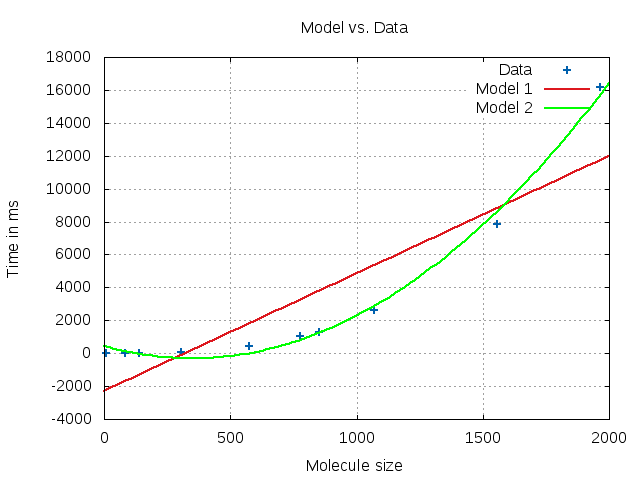
\includegraphics[width=0.8\textwidth]{images/solver-perf-model.png}
  \caption{Plot overlaying measured data with Model 1 and Model 2 (quadratic).}
\end{figure}

\begin{center}
  \begin{tabular}{ | c | c | }
    \hline
    \textbf{Model complexity} & \textbf{Coefficient of Determination ($R^2$)} \\ \hline
    \hline
        $\mathcal{O}(n^2)$ & 0.9941 \\ \hline
        $\mathcal{O}(n^3)$ & 1 \\ \hline
        $\mathcal{O}(n^4)$ & 1 \\ \hline
  \end{tabular}
\end{center}

\pagebreak

%%%%%%%%%%%%%%%%%%%%%%%%%%%%%
\section{Appendix}
%%%%%%%%%%%%%%%%%%%%%%%%%%%%%

\subsection{Hardware}

\begin{description}
    \item[Machine] \hfill \\
    System: LENOVO (portable) \\
    Product: 86147KG \\
    Version: ThinkPad T430u

    \item[CPU] \hfill \\
    Dual Core Intel Core i5-3317U CPU (-HT-MCP-) \\
    Cache: 3072 KB \\
    Flags: (lm nx sse sse2 sse3 sse4\_1 sse4\_2 ssse3 vmx) \\
    Clock Speed: 1701.00 MHz

    \item[Memory] \hfill \\
    Total Width: 64 bits \\
    Size: 8192 MB \\
    Type: DDR3 \\
    Clock Speed: 1600 MHz

    \item[Drives] \hfill \\
    Model: Samsung SSD 850 \\
    Size: 500.1GB

    \item[System] \hfill \\
    Kernel: 3.13.0-100-generic x86\_64 (64 bit) \\
    Distro: Ubuntu 14.04 trusty \\
\end{description}

\subsection{Tools}

The following software and scripts have been used to produce this protocol. Each description
includes basic version information to aid reproducibility of the results.

\subsubsection{Software}
\begin{itemize}
    \item GNUPlot Version 4.6 patchlevel 4
    \item Ruby 2.2.4p230 (2015-12-16 revision 53155) [x86\_64-linux]
    \item R version 3.3.1 (2016-06-21)
    \item TeXLive 2016.20160523-1\~{}ubuntu14.04.1
    \item Docker version 1.9.1, build a34a1d5
\end{itemize}

\subsubsection{Source Code}
\begin{itemize}
    \item Report -- \url{https://github.com/arax/fi-duvod/tree/task1-final/task1/docs}
    \item Data -- \url{https://github.com/arax/fi-duvod/tree/task1-final/task1/docs/data}
    \item Scripts -- \url{https://github.com/arax/fi-duvod/tree/task1-final/task1/scripts}
    \item Solver -- \url{https://github.com/arax/fi-duvod/tree/task1-final/task1/src/solver}
\end{itemize}

\subsubsection{Docker Images}
\begin{itemize}
    \item gcc:6.2.0 -- \url{https://hub.docker.com/_/gcc/}
    \item arax/solver-perf:30102016 -- \url{https://hub.docker.com/r/arax/solver-perf/}
    \item r-base:3.3.1 -- \url{https://hub.docker.com/_/r-base/}
\end{itemize}

\pagebreak

\subsection{Histograms}

\begin{figure}[!h]
  \centering
    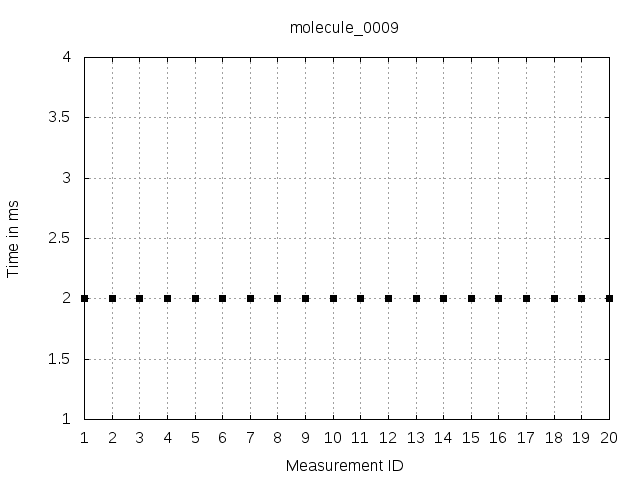
\includegraphics[width=0.8\textwidth]{images/solver-perf-molecule_0009.png}
  \caption{Measurements for a molecule of size 9.}
\end{figure}

\begin{figure}[!h]
  \centering
    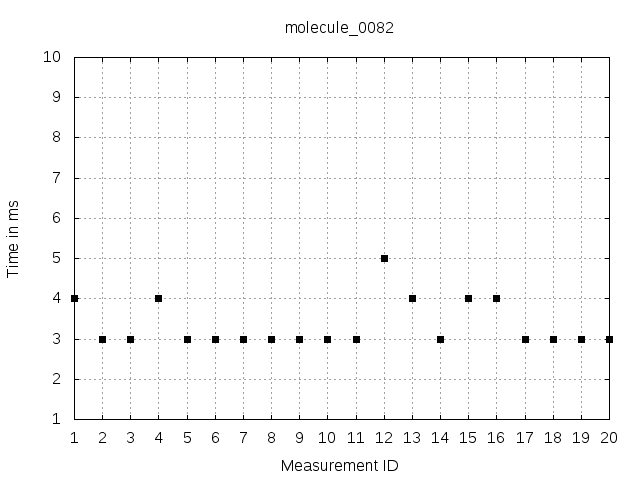
\includegraphics[width=0.8\textwidth]{images/solver-perf-molecule_0082.png}
  \caption{Measurements for a molecule of size 82.}
\end{figure}

\begin{figure}[!h]
  \centering
    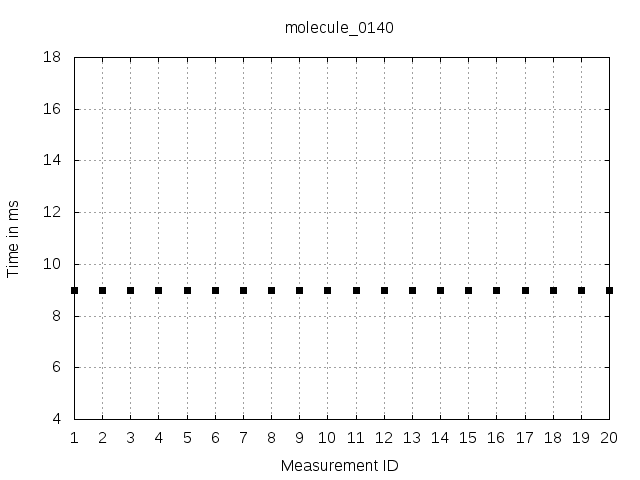
\includegraphics[width=0.8\textwidth]{images/solver-perf-molecule_0140.png}
  \caption{Measurements for a molecule of size 140.}
\end{figure}

\begin{figure}[!h]
  \centering
    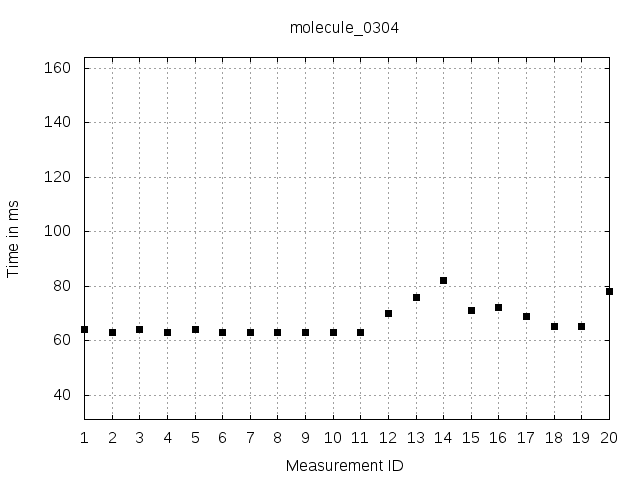
\includegraphics[width=0.8\textwidth]{images/solver-perf-molecule_0304.png}
  \caption{Measurements for a molecule of size 304.}
\end{figure}

\begin{figure}[!h]
  \centering
    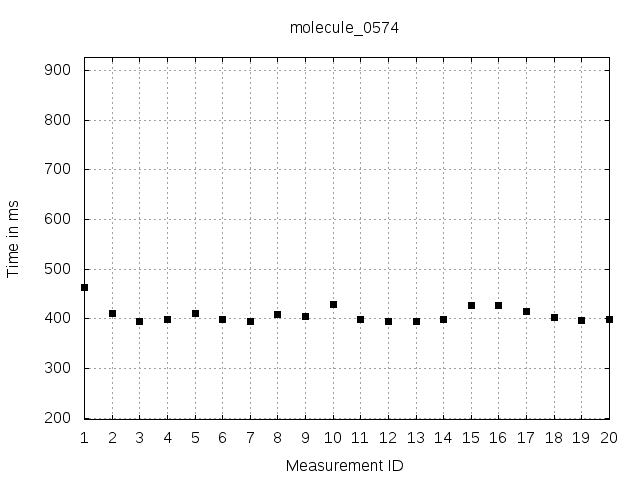
\includegraphics[width=0.8\textwidth]{images/solver-perf-molecule_0574.png}
  \caption{Measurements for a molecule of size 574.}
\end{figure}

\begin{figure}[!h]
  \centering
    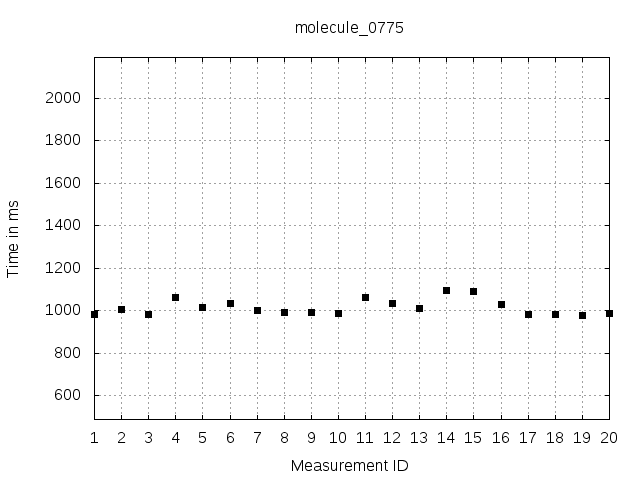
\includegraphics[width=0.8\textwidth]{images/solver-perf-molecule_0775.png}
  \caption{Measurements for a molecule of size 775.}
\end{figure}

\begin{figure}[!h]
  \centering
    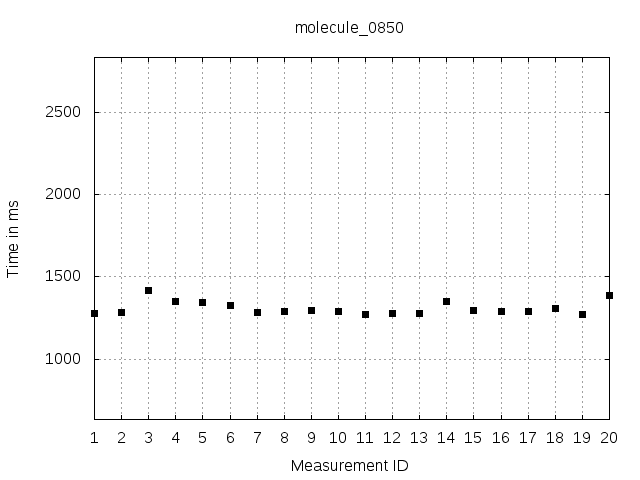
\includegraphics[width=0.8\textwidth]{images/solver-perf-molecule_0850.png}
  \caption{Measurements for a molecule of size 850.}
\end{figure}

\begin{figure}[!h]
  \centering
    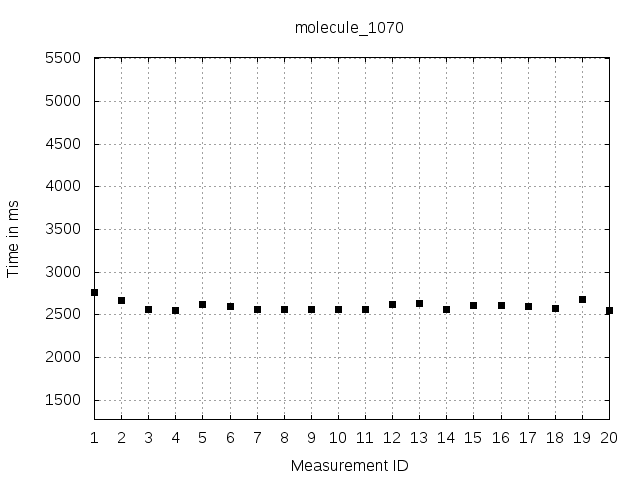
\includegraphics[width=0.8\textwidth]{images/solver-perf-molecule_1070.png}
  \caption{Measurements for a molecule of size 1070.}
\end{figure}

\begin{figure}[!h]
  \centering
    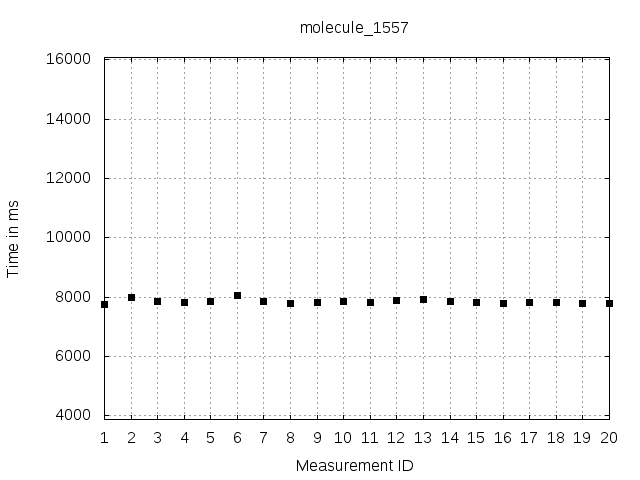
\includegraphics[width=0.8\textwidth]{images/solver-perf-molecule_1557.png}
  \caption{Measurements for a molecule of size 1557.}
\end{figure}

\begin{figure}[!h]
  \centering
    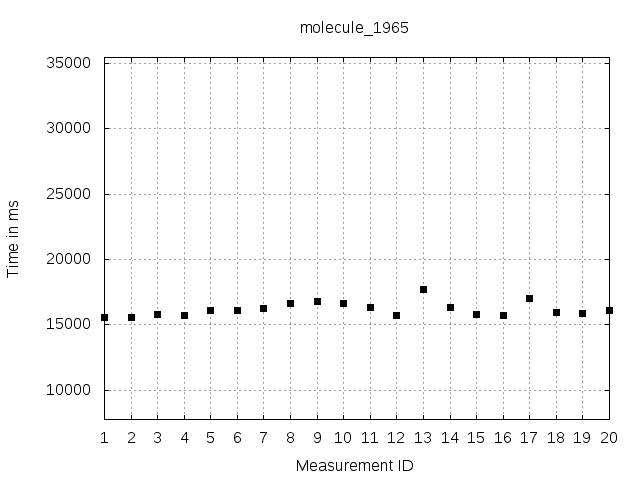
\includegraphics[width=0.8\textwidth]{images/solver-perf-molecule_1965.png}
  \caption{Measurements for a molecule of size 1965.}
\end{figure}

\end{document}
